% ==================== 2.4.6 滑移面 ====================
\subsubsection{滑移面（\texorpdfstring{$P\,1\,c\,1$}{P1c1}）}

滑移面是镜面反映与沿面内特定方向平移的联合操作，属于微观对称元素。为观察 $c$ 滑移面
（滑移方向为 $c$、滑移量为 $1/2$ 个周期），选用空间群 $P\,1\,c\,1$（No.~7，单斜
晶系，镜面垂直于 $b$ 轴），建模参数见表~\ref{tab:sym-glide}。

\begin{table}[H]
  \centering
  \caption{滑移面演示的建模参数}
  \label{tab:sym-glide}
  \begin{tabular}{ll}
    \toprule
    项目 & 参数 \\
    \midrule
    空间群 & $P\,1\,c\,1$（No.~7，单斜晶系） \\
    晶格常数 & $a=b=c=3.0$\,\AA，$\alpha=\beta=\gamma=90^\circ$ \\
    原子坐标 & Si：$(0.2,\,0.3,\,0.4)$（一般位置） \\
    等效位置数 & 2（单胞内 2 个原子） \\
    \bottomrule
  \end{tabular}
\end{table}

\begin{figure}[H]
  \centering
  \subcaptionbox{(a) 空间群与晶胞参数设置}{%
    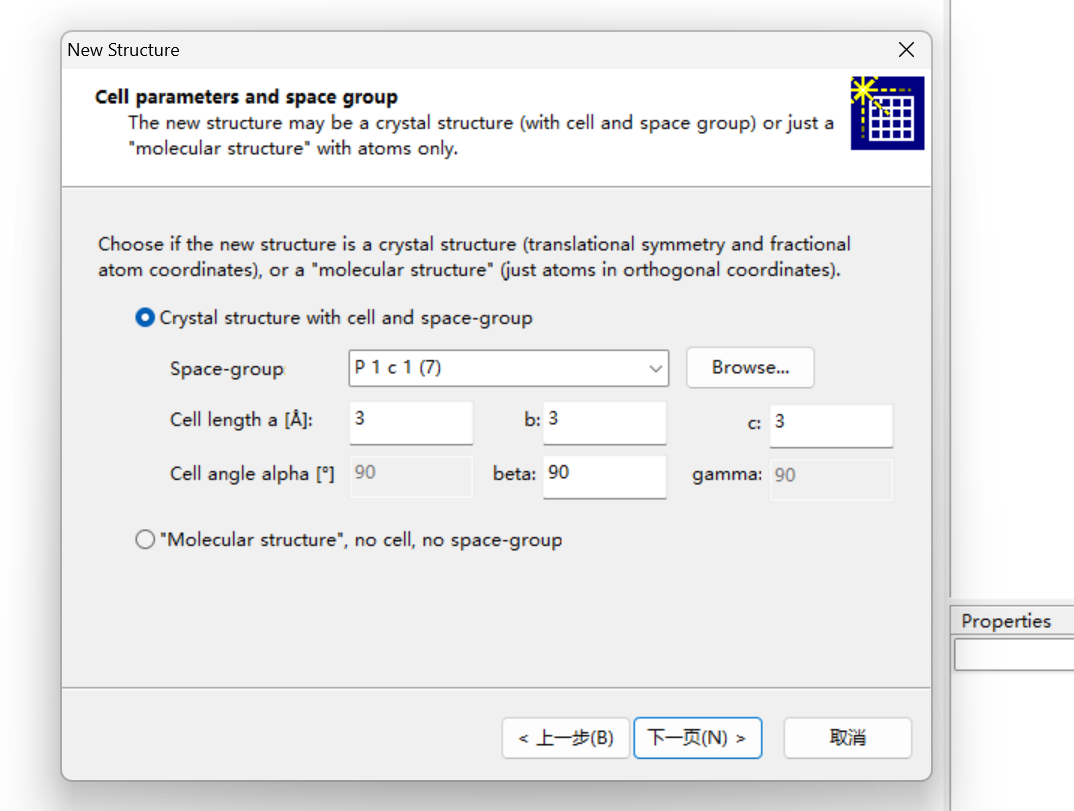
\includegraphics[width=0.44\textwidth]{assets/symmetry/glide/a.png}}
  \hfill
  \subcaptionbox{(b) 非对称单元原子（Si）添加}{%
    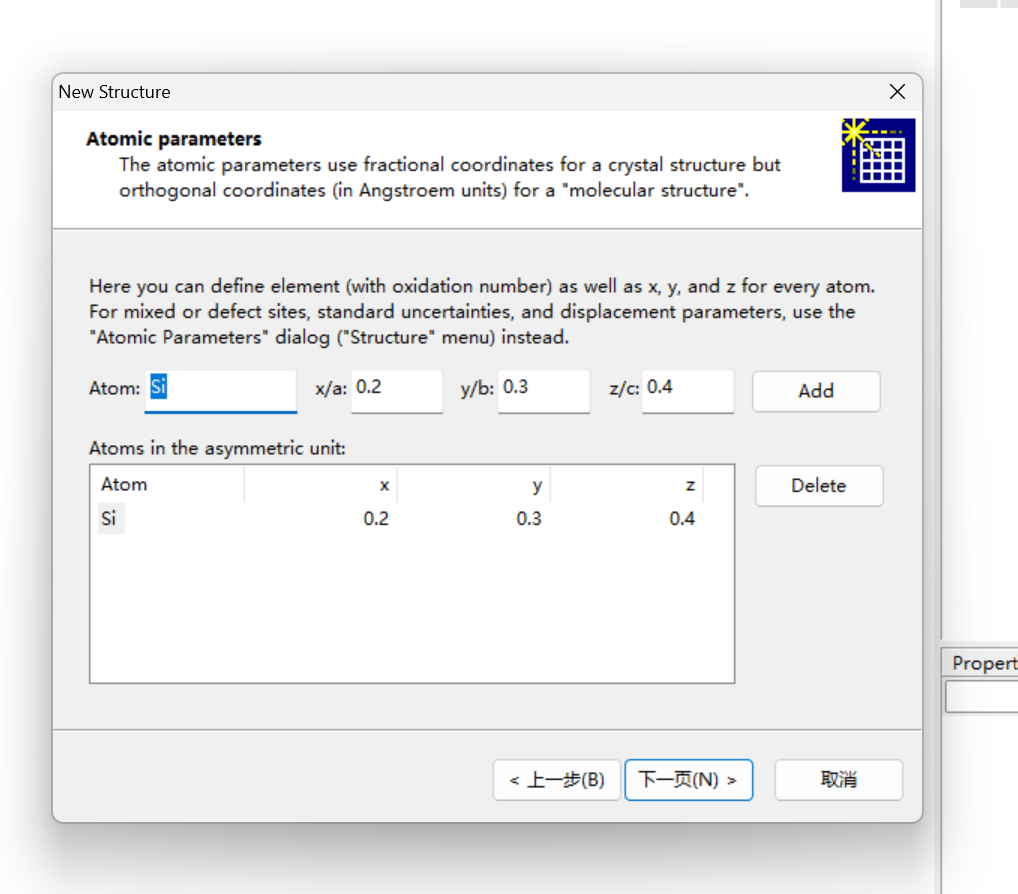
\includegraphics[width=0.44\textwidth]{assets/symmetry/glide/b.png}}
  \caption{滑移面（$P\,1\,c\,1$）演示的参数设置}
  \label{fig:sym-glide-param}
\end{figure}

\begin{figure}[H]
  \centering
  \subcaptionbox{(a) 单胞图：2 个原子由 $c$ 滑移面操作相联系}{%
    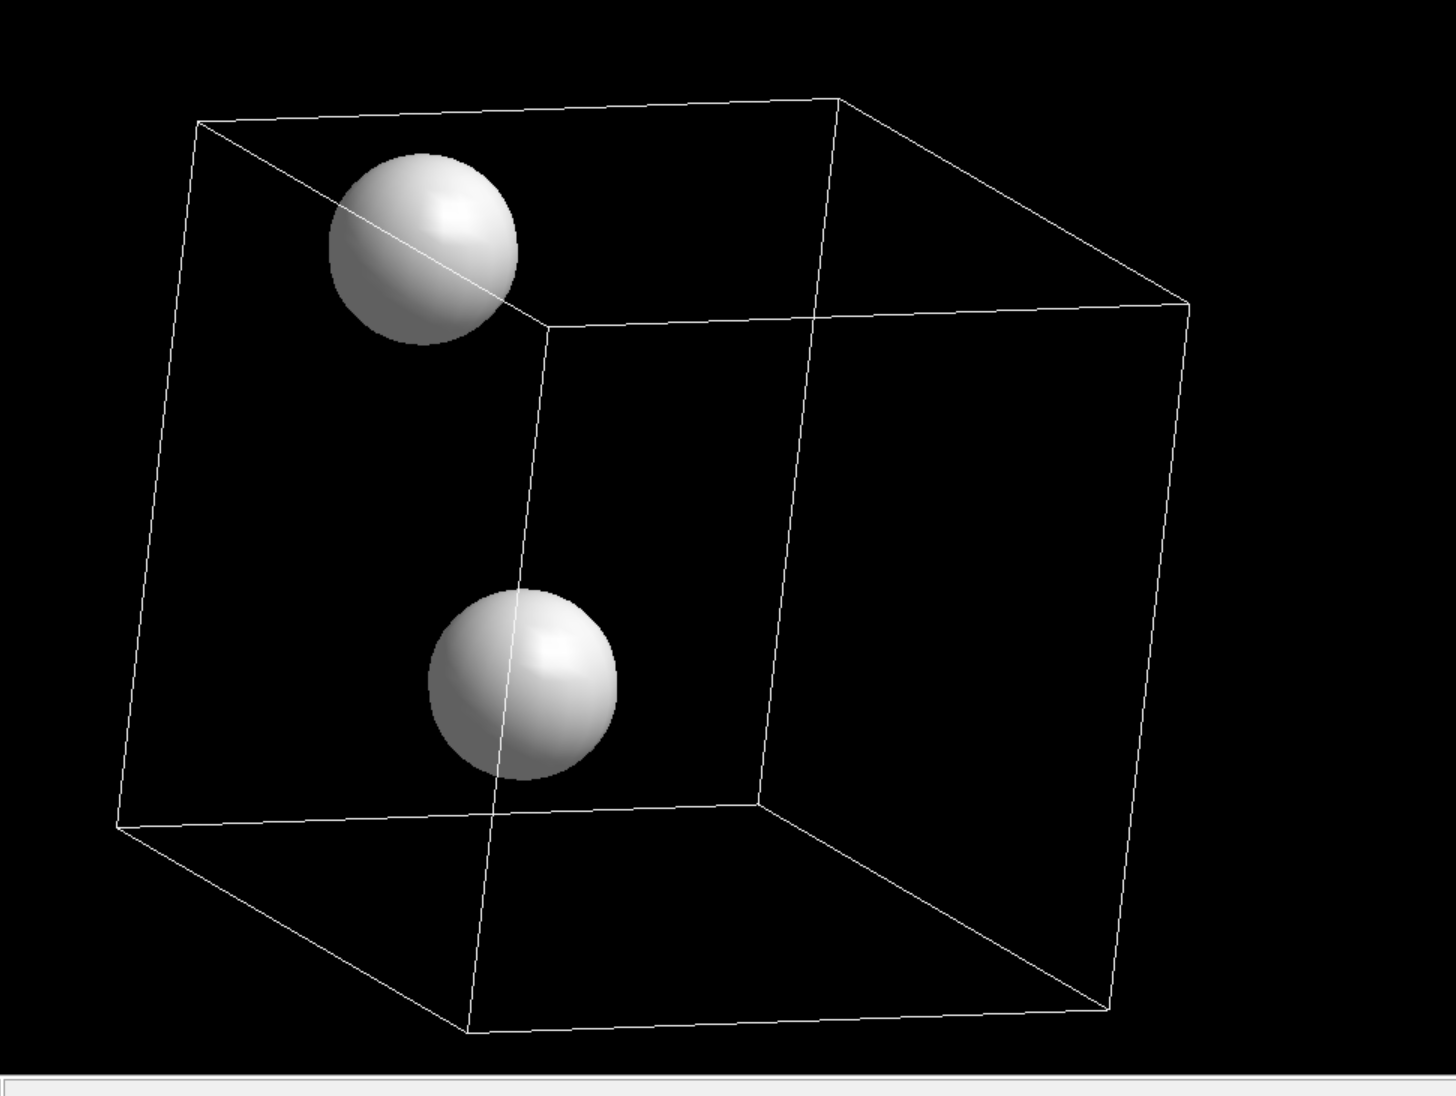
\includegraphics[width=0.44\textwidth]{assets/symmetry/glide/c.png}}
  \hfill
  \subcaptionbox{(b) 超晶胞图：相邻原子列沿 $c$ 方向错开半个周期}{%
    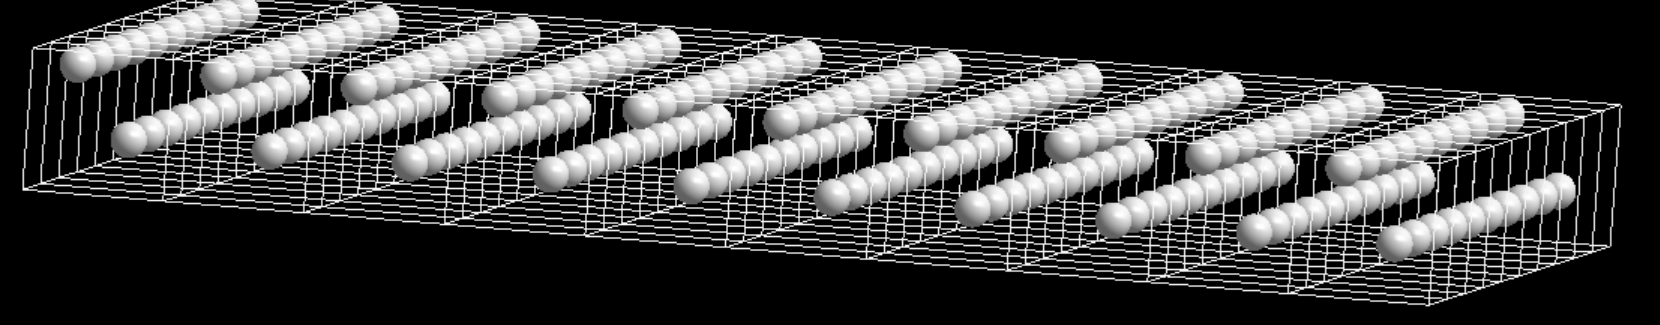
\includegraphics[width=0.44\textwidth]{assets/symmetry/glide/d.png}}
  \caption{滑移面（$P\,1\,c\,1$）的单胞与超晶胞模型}
  \label{fig:sym-glide-model}
\end{figure}

$c$ 滑移面的操作分两步：先经垂直于 $b$ 轴的镜面反映 $(x,y,z)\to(x,\bar y,z)$，再沿
$c$ 方向平移 $1/2$ 个周期，得到
\begin{equation}
  c:\quad (x,y,z)\ \longrightarrow\ (x,\,\bar y,\,z+\tfrac12)
\end{equation}
将 Si 的坐标 $(0.2,0.3,0.4)$ 代入，两个原子的分数坐标为 $(0.2,0.3,0.4)$ 与
$(0.2,0.7,0.9)$（图~\ref{fig:sym-glide-model}(a)）。在单胞中滑移操作只表现为``反映''
（两原子关于镜面等距反向），只有将模型扩展为超晶胞后，才能看到原子沿 $c$ 方向错开
半个周期的``滑移''特征：相邻原子列在 $c$ 方向上相互错位 $c/2$
（图~\ref{fig:sym-glide-model}(b)）——这正是滑移面与纯镜面的区别所在。

\textbf{特征与辨识要点。}滑移面按滑移方向分为：轴滑移面 $a$、$b$、$c$（沿相应晶轴
方向平移 $1/2$）、对角滑移面 $n$（沿面对角线方向平移 $1/2$）与金刚石滑移面 $d$
（平移 $1/4$）。滑移面含平移分量，属微观对称元素。滑移面在衍射上有确定的表现：
$c$ 滑移面垂直于 $b$ 轴时，位于 $(x,y,z)$ 与 $(x,\bar y,z+\tfrac12)$ 的两个原子对
$h0l$ 反射的散射波相位差恒为 $\pi l$，$l$ 为奇数时两者贡献恰好相互抵消——即
\textbf{$h0l$ 中 $l$ 为奇数的反射系统消光}。利用各类对称元素引起的系统消光规律判断
空间群，正是 X 射线衍射结构分析的重要内容。
